%% LaTeX template for the science justification & technical
%% feasibility to be submitted as part of a TESS Guest Investigator
%% Program proposal. This template is based on the proposal template
%% used by the NuSTAR mission.
%%
%% TESS Guest Investigator Proposal Cycle 4 template
%% V1.0
%% 2017-08-04
%% V1.1
%% 2019-02-07
%% V1.2
%% 2019-10-27
%% V1.3
%% 2020-11-02

%%%%%%%%%%%%%%%%%%%%%%%%%%%
%%%%% DOCUMENT FORMAT %%%%%
%%%%%%%%%%%%%%%%%%%%%%%%%%%

%% The default font was chosen to be easily readable while allowing
%% sufficient material to be included.

%% Please note that the proposal will be printed on US Letter size paper,
%% 8.5 in x 11 in, and that formatting the text for other sizes will
%% generally cause layout problems and may result in text being cut
%% off near the edges. PLEASE DO NOT CHANGE THE 'LETTERPAPER' OPTION
%% IN THE DOCUMENTCLASS COMMAND.

%%%%%%%%%%%%%%%%%%%%%%%%%%%%%%%%%%%%%%%%%%%%%%
%%%%% Default format: 12pt single column %%%%%
%%%%%%%%%%%%%%%%%%%%%%%%%%%%%%%%%%%%%%%%%%%%%%


%% Minimum margin size is 1 inch from top, bottom, and sides.
%% Font size: see NASA Guidebook for Proposers 
%%(https://www.hq.nasa.gov/office/procurement/nraguidebook/proposer2018.pdf).

\documentclass[letterpaper,12pt]{article}

%%%%%%%%%%%%%%%%%%%%%%%%%%%%%%%%%%
%%%%% HOW TO INCLUDE FIGURES %%%%%
%%%%%%%%%%%%%%%%%%%%%%%%%%%%%%%%%%

%% Please see the ``Included packages'' section below.

%%%%%%%%%%%%%%%%%%%%%%%%%%%%%
%%%%% Included packages %%%%%
%%%%%%%%%%%%%%%%%%%%%%%%%%%%%

\usepackage{graphics,graphicx}
\usepackage[colorlinks]{hyperref}
\hypersetup{urlcolor=blue}
\usepackage{cleveref}
\usepackage{natbib}

%% Feel free to modify the included packages list to use your
%% favorite packages. 

%% In the graphics and graphicx packages, Postscript and eps figures
%% can be included using the \includegraphics command. The graphics
%% package is part of standard LaTeX2e and provides a basic way of including a
%% figure. The graphicx package is not standard, but extends the
%% \includegraphics command to make it more user-friendly. If graphicx
%% is not available on your system please remove it from the list of
%% included packages above.  

%% Syntax:
%% In the graphics package:
%%
%% \begin{figure}
%% \includegraphics[llx,lly][urx,ury]{file}
%% \end{figure}
%%
%% where ll denotes 'lower left' and ur 'upper right' and the x and y
%% values are the coordinates of the PostScript bounding box in
%% points. There are 72 points in an inch.
%%
%% In the graphicx package:
%% 
%% \begin{figure}
%% \includegraphics[key=val,key=val,...]{file}
%% \end{figure}
%%
%% where some of the useful keys are: angle, width, height,
%% keepaspectratio (='true' or 'false') and scale. Bounding box values
%% can be given as [bb=llx lly urx ury].
%%
%% In either case you have to use LaTeX figure placement commands to
%% position the figure on the page; \includegraphics will not do
%% that. Both these commands also have other options that are listed
%% in the LaTeX manual (for the graphics package) and in 'The LaTeX
%% Graphics Companion' (for the graphicx package).



%%%%%%%%%%%%%%%%%%%%%%%%%%%
%%%%% Page dimensions %%%%%
%%%%%%%%%%%%%%%%%%%%%%%%%%%

\setlength{\textwidth}{6.5in} 
\setlength{\textheight}{9in}
\setlength{\topmargin}{-0.0625in} 
\setlength{\oddsidemargin}{0in}
\setlength{\evensidemargin}{0in} 
\setlength{\headheight}{0in}
\setlength{\headsep}{0in} 
\setlength{\hoffset}{0in}
\setlength{\voffset}{0in}



%%%%%%%%%%%%%%%%%%%%%%%%%%%%%%%%%%
%%%%% Section heading format %%%%%
%%%%%%%%%%%%%%%%%%%%%%%%%%%%%%%%%%

\makeatletter
\renewcommand{\section}{\@startsection%
{section}{1}{0mm}{-\baselineskip}%
{0.5\baselineskip}{\normalfont\Large\bfseries}}%
\makeatother

%%%%%%%%%%%%%%%%%%%%%%%%%%%%%%%%%%%%%
%%%%% Some Useful Abbreviations %%%%% 
%%%%%%%%%%%%%%%%%%%%%%%%%%%%%%%%%%%%%
\newcommand{\tess}{{\it TESS}}
\newcommand{\jwst}{{\it JWST}}
\newcommand{\kepler}{{\it Kepler}}
\newcommand{\spitzer}{{\it Spitzer}}
\newcommand{\ktwo}{{K2}}
\newcommand{\hst}{{\it HST}}
\newcommand{\swift}{{\it Swift}}
\newcommand{\integral}{{\it INTEGRAL}}
\newcommand{\nustar}{{\it NuSTAR}}
\newcommand{\fermi}{{\it Fermi}}
\newcommand{\mum}{\ifmmode{\rm \mu m}\else{$\mu$m}\fi}
\newcommand{\ms}{$M_{\odot}$}
\newcommand{\rs}{$R_{\odot}$}
\newcommand{\ls}{$L_{\odot}$}
\newcommand{\re}{$R_{\oplus}$}
\newcommand{\me}{$M_{\oplus}$}
\newcommand{\kms}{km~s$^{-1}$}
\newcommand{\fluxcgs}{ergs~s$^{-1}$~cm$^{-2}$}
\newcommand{\lumcgs}{ergs~s$^{-1}$}
\newcommand{\rj}{$R_{\textrm{\scriptsize Jup}}$}
\newcommand{\mj}{$M_{\textrm{\scriptsize Jup}}$}
\newcommand{\mnras}{MNRAS}
\newcommand{\apjl}{ApJL}
\newcommand{\apj}{ApJ}
\newcommand{\nat}{Nature}
\newcommand{\pasp}{PASP}

%%%%%%%%%%%%%%%%%%%%%%%%%%%%%
%%%%% Start of document %%%%% 
%%%%%%%%%%%%%%%%%%%%%%%%%%%%%

\begin{document}
\pagestyle{plain}
\pagenumbering{arabic}


 
%%%%%%%%%%%%%%%%%%%%%%%%%%%%%
%%%%% Title of proposal %%%%% 
%%%%%%%%%%%%%%%%%%%%%%%%%%%%%

\begin{center} 
\bfseries\uppercase{%
%%
%% ENTER TITLE OF PROPOSAL BELOW THIS LINE
MONITORING THE JWST SPECTRO-PHOTOMETRIC STANDARDS
%%
%%
}
\end{center}



%%%%%%%%%%%%%%%%%%%%%%%%%%%%%%%%%%%%%%%%%
%%%%% Body of science justification %%%%%
%%%%% and technical feasibility     %%%%%
%%%%%%%%%%%%%%%%%%%%%%%%%%%%%%%%%%%%%%%%%


%%%%%%%%%%%%%%%%%%%%%%%%%%%%%%%%%%%%%%%%%
%%%%%%%%%%%%%%%%%%%%%%%%%%%%%%%%%%%%%%%%%
%%%%% The text below should be commented out before submitting your proposal %%%%% 
% \noindent{The recommended sections for a \tess\ GI proposal are shown below. Feel free to change section 
% headings as necessary, but this is the suggested minimal information that should be included in the proposal. 
% This Science/Technical section of the proposal is limited to 2 pages. Figures are included in these page limits, but not references or a (sample) target table. \\

% \noindent Note that the Phase-1 proposal review will be done in a dual-anonymous fashion and follow the guidelines listed below:
% \begin{itemize}
%     \item Proposals should eliminate language that identifies the proposers or institution, as discussed in the \href{https://science.nasa.gov/researchers/dual-anonymous-peer-review}{Guidelines for Anonymous Proposals}.
%     \item PIs are required to upload a one-page Team Expertise (insert link) PDF through a separate upload when submitting the science justification into ARK/RPS.
%     \item Proposals that do not follow these dual-anonymous guidelines may be returned without review.
% \end{itemize}

% \noindent Mini proposals are intended for requests for a small number of target slots and require minimal resources, up to 50 20-second cadence targets and 1,000 2-minute cadence targets. Proposals in this category are not eligible for funding.\\ 

% \noindent Mini proposals cannot have Targets of Opportunity, a joint component with \hst, \swift, or \fermi, or have a ground-based component. 
%  } 
%%%%% The text above should be commented out before submitting your proposal %%%%% 
%%%%%%%%%%%%%%%%%%%%%%%%%%%%%%%%%%%%%%%%%
%%%%%%%%%%%%%%%%%%%%%%%%%%%%%%%%%%%%%%%%%


%This will be removed and added to the submission form. Avoid latex.
%\section{Abstract}
%We propose to use the TESS 2-minute cadence to monitor the James Webb Space Telescope (JWST) spectro-photometric standard stars for unexpected variability. These stars are necessary to accurately calibrate the absolute and relative flux JWST receives across its range of infrared wavebands. The standard star list used by JWST include white dwarf stars, and main sequence stars of spectral type B9 to G1. By monitoring these stars with TESS at a 2-minute cadence we will be able to determine if the star has recently shown evidence of brightness variations due to flares, pulsations or stellar spots. Additionally, we will also be able to check that each star has not recently undergone occultations from planets or dust, as seen for some white dwarf stars. For some stars we can check for evidence of long term variations like recently seen in Betelgeuse. By monitoring these stars with TESS at a short cadence we add to our understanding of the stability of the stars and thereby enable the JWST calibrations team to provide the best spectro-photometric calibrations of the JWST data. 


 %REMINDER:  THIS NEEDS to be written anonymously
\section{Scientific Justification and Perceived Impact}

The James Webb Space Telescope (\jwst) will launch in October 2021 and revolutionize our view of all areas of astrophysics, from exoplanets to the formation of Galaxies. To accomplish these goals, \jwst\ will observe a sample of spectro-photometric standard stars in order to achieve an absolute flux calibration with the goal of better than 2\% accuracy.  The calibration stars are chosen because they have well-known absolute fluxes and spectral shapes across the \jwst\ wavelength range, 0.6--28.5 \mum.  The success of this program will not only enable the cross-instrument calibration of the \jwst\ science instruments, but also tie \jwst\ to \hst, \spitzer, and other ground-based telescopes \citep{Bohlin2014PASP}.

The \jwst\ science programs span all areas of science from the outer solar system, to exoplanet atmospheres, stellar nurseries, and the formation of the first Galaxies. Any science program that will combine infrared spectra and photometry from \jwst\ to other telescopes will require a precise understanding of the flux received by the \jwst\ instruments.  Even those looking to combine spectra and photometry across different \jwst\ instruments and modes will need to address the relative sensitivities of these instruments. If the standard stars vary in any way between exposures, the flux calibration could be systematically off. While using a suite of stars mitigates against obvious outliers, monitoring standards for any variability will improve the calibration team's understanding of which stars are possible outliers and thereby establish the best possible calibration for \jwst\ data.  

%the calibration ensuring that the stars are not variable during  of the c As a simple example, those looking for evidence of a dust disk from infrared excesses will want to compare the photometry across all of the JWST bands.  Something with Galaxies....something with exoplanets....\textit{Short paragraph on science programs that require accurate photometry to emphasize the impact}

%The JWST calibration program is performed by observing NN stars with various instruments ... \textit{Describe how photometric standards are used emphasizing our assumptions about photometric stability}
%Even some white dwarfs, which are frequently used as standards, can show dynamic variability due to magnetic fields, pulsations and binarity \citep{Hermes2017}.

Time series missions like \tess\ and \kepler\ have taught us that stars can vary in brightness for a variety of reasons at a variety of time scales \citep{Hermes2017}. Pulsating stars exist across the HR diagram and have periods from years to minutes. Many stars show evidence of stellar activity which manifests as stellar spots and unexpected flares. Other stars change brightness because of dust, planets or binarity.  Cautionary tales of unexpected variations in stars are now common in the literature, for example: 
\begin{itemize}
    \item  Boyajian's star, KIC~8462852 \citep{Boyajian2016}, was discovered using \kepler\ data, and it shows unexplained drops in flux as large as 20\% at random times.
    \item Several triple star systems were identified in the \kepler\ data \citep{Orosz2015} where eclipses appeared and disappeared following third body fly-bys. 
    \item The nearby red supergiant Betelgeuse \citep{Guinan2019} dimmed by more than 1 visual magnitude in 2019, the deepest decline reported in 50 plus years of observations \citep{Levesque2020ApJ}.
    \item Some white dwarfs show random or pseudo-periodic dips in brightness caused by disintegrating planets. These dips are as large as 40\% and only last a few minutes \citep{Vanderburg2015}.
    \item The pulsating white dwarf GD~358 suddenly changed the period and amplitude of its pulsations \citep{Montgomery2010}, showing that even predictable pulsations can suddenly change.
\end{itemize}

While ideally the \tess\ observations would occur at the same time as the \jwst\ observations, neither mission has flexibility in its scheduling to make that possible.  However, because \tess\ Cycle 4 overlaps the first cycle of \jwst\ science time, the observations will occur within a few months of each other, allowing the best chance to see the ``current'' state of the star's variability. Also, because \tess\ is able to observe in the infrared, like \jwst, the observed amplitudes of any variability will match those seen by \jwst.

We request monitoring with two-minute cadences for these stars to ensure we have the time resolution required to find and understand any variability that could impact the use of a star as a standard. The exposure times for the calibration stars are as small as a few minutes and probe flux variations on this time scale. To thoroughly probe these objects as standard stars, we require a cadence that will equal or surpass that of the exposure times - this is especially important for pulsating stars where the Nyquist frequency (half the sampling rate) dictates which pulsations are visible.
%Stellar flares, pulsations and occultations have all been detected on this time scale and could be missed at the ten-minute cadence.

To further emphasize the importance of this monitoring, an initial review of existing \tess\ data has revealed variability in a few of the listed spectro-photometric standards.  Figure~\ref{fig:lc} shows the light curve of the standard star HD~38949 (TIC 32869782) shows peak-to-peak variations of 1\% at a period of $\sim$7 days. 

If successful, by the end of Cycle 4 there will be 2-minute \tess\ observations for a majority of the \jwst\ calibration stars, with thirty-one of them having observations taken within a few months of the \jwst\ calibration program. These data will provide important evidence about the variable nature of the star and will aide the \jwst\ calibration team to achieve the highest quality spectro-photometric calibrations.

%While in most cases the amplitudes of the pulsations are likely not large enough to impact the \jwst\ calibrations, these \tess\ observations will help us better understand the stellar astrophysics that can impact the star's ability to act as a spectro-photometric standard.

\begin{figure}
    \centering
    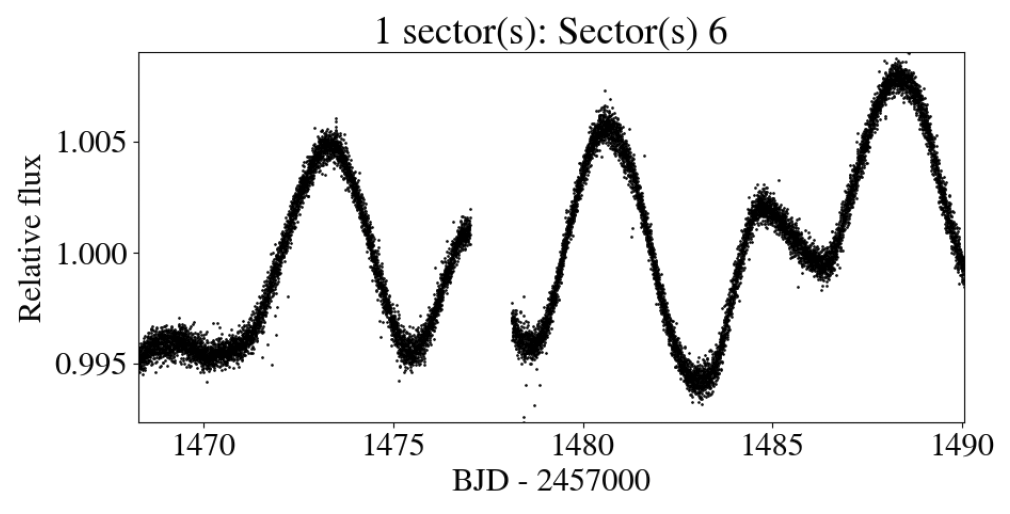
\includegraphics[scale=.5]{HR38949_lc.png}
    \caption{\tess\ sector 6 light curve of the \jwst\ calibration star, HD 38949 (TIC~32869782).}
    \label{fig:lc}
\end{figure}


%Provide text and figures that justify the scientific need for new \tess\ observations and analyses here. In particular, justify your choice of new 2~min or 20~s cadence observations. If you will also be making use of the 10~min FFIs for your research, make it clear why the \tess\ FFI data are suitable for your science.

%Summarize the expected science return of the proposed investigations and the expected benefit to the community.


\section{Analysis Plan and Technical Feasibility}
Thirty-one \jwst\ spectro-photometric standards are observable during \tess\ Cycle 4, six of which have less than two sectors of any existing TESS observations. Our target list prioritizes those with the fewest TESS sectors already in the archive. The targets range in \tess\ magnitudes from 4 to 16 yielding a photometric precision ranging from 0.006\% to 0.15\%, with significantly higher precision for periodic phenomena.  We plan to analyze the variability of these targets using the Lightkurve software package \citep{2018ascl.soft12013L}. We will look for both periodic variability and sudden changes in brightness using a variety of detection methods including periodograms, transit search algorithms and visual inspection. We will examine the crowding of each target to adjust the amplitudes of any observed variability. Finally, we will report the photometric limits, or any detected variability, in a refereed paper.


\clearpage

\bibliography{references}{}
\bibliographystyle{abbrv}
%List of references. References {\it are {\bf not} included} when considering the proposal page limit. References in the text should be in the number format, and in the references list as:

%[1] Person A, Person B, Person C, et al., 2016, ApJ 200, 231, 2\\
%[2] Person D \& Person E, 1912, Nature 495, 452


%\section{Target Table}

%When necessary to justify your proposal, provide a list of targets using the below example as a template for format. This target table is designed to aid reviewers and need only provide a representative sample of the complete target list uploaded to RPS. Full target tables should be submitted electronically with the Phase-1 proposal. Please limit any target table included here to only 1 page. The table is not included in the page limit of the Science/Technical section. 


\section{ Three Example Targets}
\begin{center}
\begin{tabular}{ | c | c | c | c | c | c | c | }

\hline
TIC ID          &      Common      &     RA             &      Dec          &      TESS       &       Obj.        &      Comments \\       
                    &      Name           &     (deg)          &      (deg)        &      mag         &       Type       &                         \\     
\hline
\hline
381024911 & ksi2 Cet & 37.0398 & 8.46006 & 4.328 & B9III & 2-min\\ \hline
352817378 & LDS 749B & 323.0676365 & 0.253999538 & 14.778 & DBQ4 & 2-min\\ \hline
397558558 & HD 106252 & 183.3729584	 & 10.04163578 & 6.85 & G0 & 2-min \\ \hline


\end{tabular}
\end{center}   

%%%%%%%%%%%%%%%%%%%%%%%%%%%
%%%%% End of document %%%%%
%%%%%%%%%%%%%%%%%%%%%%%%%%%

\end{document}

